%!TEX root = bachelor.tex
\chapter{Analyse}
\label{ch:analysis}
In diesem Kapitel bla bla bla.


\section{Vergleich Vorwärtsentfaltung und Rückwärtsentfaltung}

Bla bla Rückwärtsentfaltung ist optisch viel besser und schneller, deshalb beziehen sich alle folgenden Analysen nur noch auf Rückwärts
wenn man umkerabbildung bestimmen kann ist das vorzuziehen
warum kann man nicht richtig vergleichen


\begin{figure}[!htb]
	\centering
	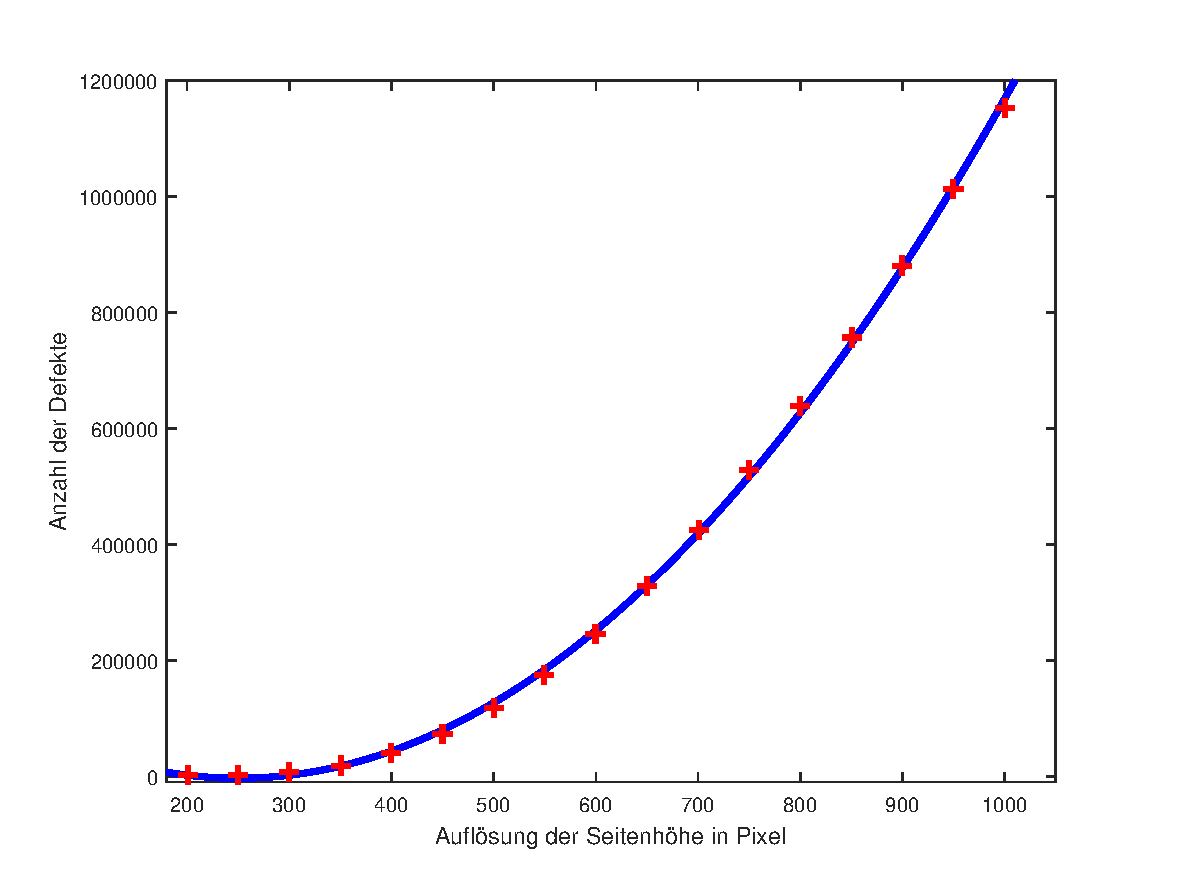
\includegraphics[width=\textwidth]{images/numberOfHoles.eps}
	\caption{Einfluss der Ausgabeauflösung auf die Anzahl der Löcher}
	\label{fig:influenceRes}
\end{figure}

\section{Einfluss der intrinsischen Kalibrierung}

\begin{figure}[!htb]
	\centering
	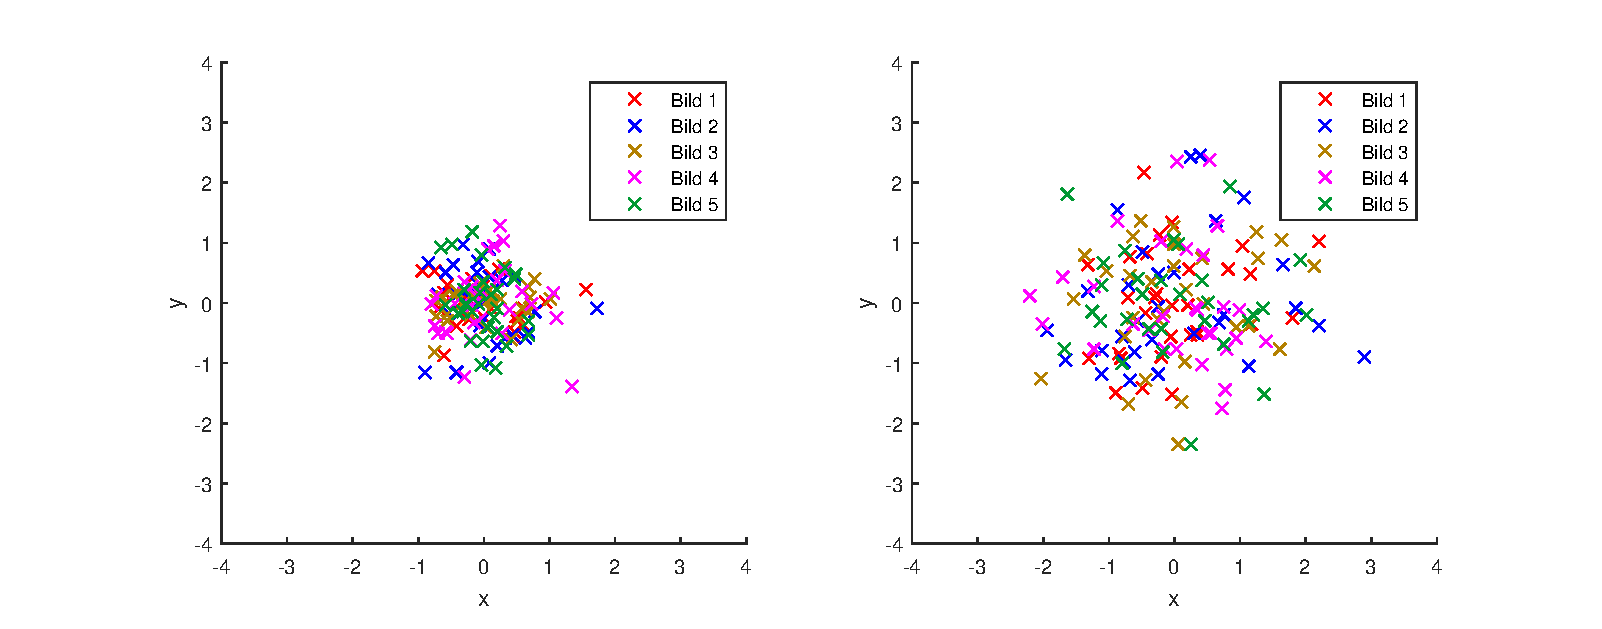
\includegraphics[width=\textwidth]{images/reprojectionErrorReverse.eps}
	\caption{Einfluss der intrinsischen Kalibrierung}
	\label{fig:influenceCalib}
\end{figure}

prjektionsfehler ohne kalib ist wesentlich größer, da die implizitie intrinsiche kalib durch die svd keine verzerrung entfernt

\section{Einfluss der Rotation der Kamera}
Um den Einfluss der Rotation der Kamera zu untersuchen, wurde der Kegel mit Kalibrierungsmuster in Blender gerendert, da die Kameraposition dann genau bekannt ist und äußere Faktoren wie Lichtverhältnisse und inhomogene Hintergründe kontrolliert werden können. 

\begin{figure}[!htb]
	\centering
	\begin{subfigure}{.5\textwidth}
		\centering
		\includegraphics[width=.9\textwidth]{images/blender0.png}
		\caption{bei 0°}
	\end{subfigure}%
	\begin{subfigure}{.5\textwidth}
		\centering
		\includegraphics[width=.9\textwidth]{images/blender12.png}
		\caption{bei 12°}
	\end{subfigure}
	\label{fig:blender}
	\caption{gerendeter Kegel mit Kalibrierungsmuster in Blender}
\end{figure}


Es werden anschließend Bilder erzeugt, in denen in 1° Schritten die Kamera von 0° bis 12° um die $X$-Achse rotiert wird. Für jedes dieser Bilder wird anschließend eine Rückwärtsentfaltung durchgeführt und der Reprojection-Fehler bestimmt. Abbildung \ref{fig:influenceRot} zeigt, dass der Reprojection-Fehler rotationsinvariant ist. 


\begin{figure}[!htb]
	\centering
	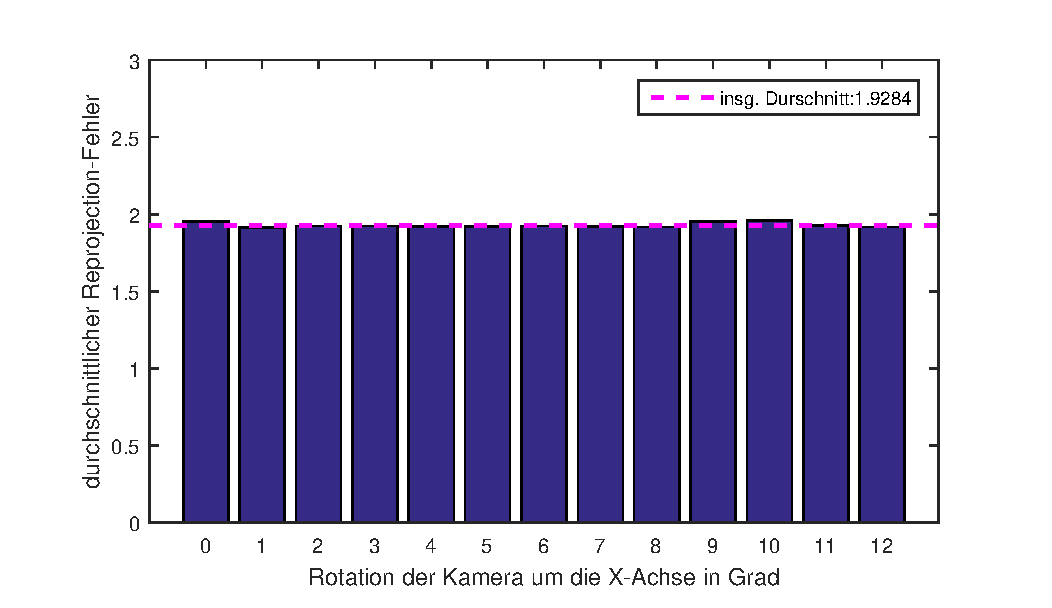
\includegraphics[width=\textwidth]{images/reprojectionErrorDeg2.eps}
	\caption{Einfluss der Rotation der Kamera}
	\label{fig:influenceRot}
\end{figure}





\section{Laufzeit der Entfaltung}

Raspberry Pi 2 Model B:
\begin{itemize}
	\item 900MHz ARM Cortex-A7 CPU
	\item 1GB RAM
	\item GCC-4.??? Release
	\item Opencv 2.4.13
\end{itemize}

\begin{figure}[!htb]
	\centering
	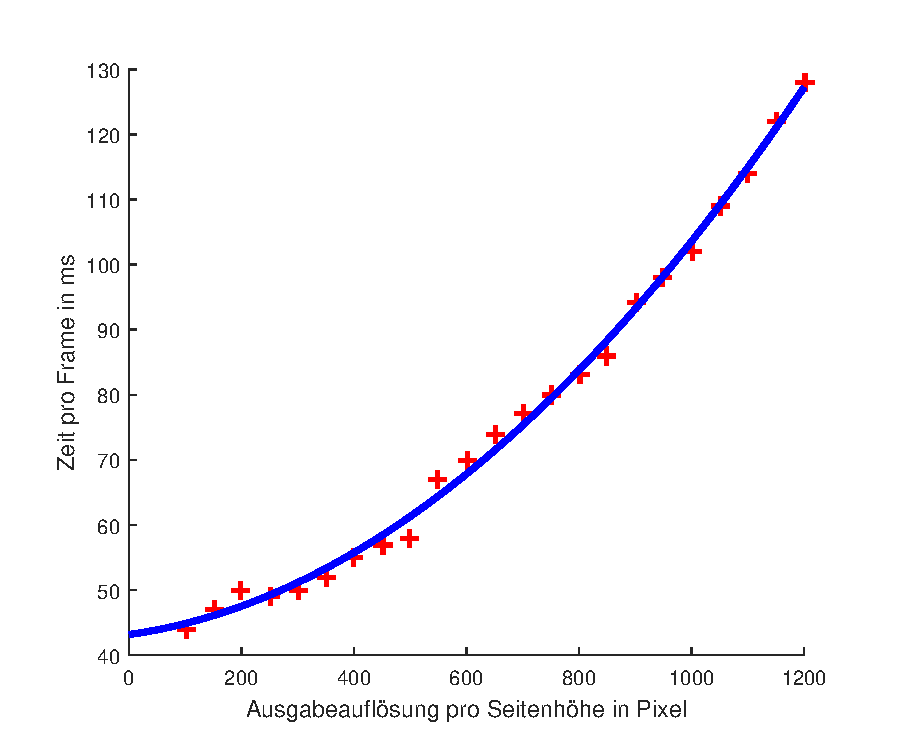
\includegraphics[width=\textwidth]{images/runningTimePerSlantheight.eps}
	\caption{Einfluss der Ausgabeauflösung auf die Laufzeit}
	\label{fig:influenceRes2}
\end{figure}




\bigskip\bigskip

projektionsfehler bei dem einen
anzahl löcher bei dem anderen



robustheit reverse warping? bestimmung der keypoints?







\section{Evaluierung des RANSAC zur Ellipsendetektion}



\begin{figure}[!htb]
	\centering
	\begin{subfigure}{.5\textwidth}
		\centering
		\includegraphics[width=.9\textwidth]{images/ransac50_0.png}
		\caption{gestörte Messdaten}
	\end{subfigure}%
	\begin{subfigure}{.5\textwidth}
		\centering
		\includegraphics[width=.9\textwidth]{images/ransac50_1.png}
		\caption{detekt. Ellipsen: RANSAC (grün), LSQ (cyan)}
	\end{subfigure}
	\label{fig:bla}
	\caption{Vergleich RANSAC und LSQ bei gleichverteilten Ausreißern $\epsilon = 0.5, p = 0.99$}
\end{figure}

\begin{figure}[!htb]
	\begin{subfigure}{.5\textwidth}
		\centering
		\includegraphics[width=.9\textwidth]{images/ransacShadow25_0.png}
	\end{subfigure}%
	\begin{subfigure}{.5\textwidth}
		\centering
		\includegraphics[width=.9\textwidth]{images/ransacShadow25_1.png}
	\end{subfigure}
	\begin{subfigure}{.5\textwidth}
		\centering
		\vspace{0.2cm}
		\includegraphics[width=.9\textwidth]{images/ransacShadow40_0.png}
	\end{subfigure}%
	\begin{subfigure}{.5\textwidth}
		\centering
		\vspace{0.2cm}
		\includegraphics[width=.9\textwidth]{images/ransacShadow40_1.png}
	\end{subfigure}
	\caption{Vergleich RANSAC und LSQ bei Schattenellipsen mit $p = 0.99$ und $\epsilon = 0.25$ (oben), $\epsilon = 0.4$ unten, links gestörte Messdaten, rechts detektierte Ellipsen RANSAC (grün), LSQ (cyan)}
	\label{fig:blubb}
\end{figure}























